% ------------------------------------------------------------
% Relatório Técnico LeadScore AI – Versão Melhorada
% ------------------------------------------------------------
\documentclass[portuguese,11pt]{article}
\usepackage[utf8]{inputenc}
\usepackage[margin=1in]{geometry}
\usepackage{amsfonts,amsmath}
\usepackage{forest}
\usepackage{graphics,graphicx}
\usepackage{listings}
\usepackage[T1]{fontenc}
\usepackage{fullpage}
\usepackage{indentfirst}
\usepackage{colortbl}
\usepackage[inline]{enumitem}
\usepackage[colorlinks=true, allcolors=black]{hyperref}
\usepackage[nameinlink, noabbrev]{cleveref}
\usepackage{eso-pic}
\usepackage{float}
\usepackage[skip,indent]{parskip}
\usepackage{caption,subcaption}
\setlength{\parskip}{2pt}
\usepackage{xcolor}
\usepackage{pgfgantt}
\usepackage{hyperref}
\usepackage{colortbl}
\usepackage{booktabs}
\usepackage{fontawesome}

\usepackage{colortbl}
\usepackage{textgreek}

% ------------------------------------------------------------
% Cores personalizadas
% ------------------------------------------------------------
\definecolor{codegreen}{rgb}{0,0.6,0}
\definecolor{codegray}{rgb}{0.5,0.5,0.5}
\definecolor{codepurple}{rgb}{0.58,0,0.82}
\definecolor{backcolour}{rgb}{0.95,0.95,0.92}

\lstdefinestyle{mystyle}{%
    backgroundcolor=\color{backcolour},
    commentstyle=\color{codegreen},
    keywordstyle=\color{magenta},
    numberstyle=\tiny\color{codegray},
    stringstyle=\color{codepurple},
    basicstyle=\ttfamily\small,
    breaklines=true,
    captionpos=b,
    keepspaces=true,
    numbers=left,
    numbersep=5pt,
    showspaces=false,
    showstringspaces=false,
    showtabs=false,
    tabsize=2}
\lstset{style=mystyle,inputencoding=utf8}

\newcommand{\hsp}{\hspace{20pt}}
\newcommand{\HRule}{\rule{\linewidth}{0.5mm}}
\newcommand{\rev}[1]{\textcolor{red}{#1}}

% ------------------------------------------------------------
% Documento
% ------------------------------------------------------------
\title{LeadScore AI - Sistema Inteligente de Priorização de Leads}
\date{Outubro 2025}

\begin{document}

% ------------------------------------------------------------
% Página de título
% ------------------------------------------------------------
\begin{titlepage}
  \begin{center}
    \vspace*{2cm}
    \textsc{\Large Relatório de Implementação - Aprix Software Solutions}\\[0.5cm]
    \HRule \\[0.4cm]
    {\huge \bfseries LeadScore AI\\[0.2cm]
    Sistema Inteligente de Priorização de Leads\\[0.4cm]}
    \href{https://github.com/LucasTramonte/LeadScore-AI-Lead-Prioritization-System}{\faGithub\, Repositório GitHub LeadScore AI}
    \HRule \\[1cm]
    \vfill
    {\large Outubro 2025}
  \end{center}
\end{titlepage}

\tableofcontents
\newpage

% ------------------------------------------------------------
% Resumo Executivo
% ------------------------------------------------------------
\section*{Resumo Executivo}
\addcontentsline{toc}{section}{Resumo Executivo}

\subsection*{O Desafio Empresarial}
A Aprix enfrentava um desafio crítico na gestão de seu funil de vendas. Com centenas de leads chegando mensalmente através de diferentes canais, a equipe comercial não possuía critérios objetivos para identificar quais prospects apresentavam maior probabilidade de conversão. Esta situação resultava em ineficiências operacionais significativas, incluindo tempo desperdiçado com leads de baixo potencial, oportunidades de alto valor sendo negligenciadas por falta de priorização adequada, e inconsistência na abordagem de qualificação entre diferentes membros da equipe de vendas.

\subsection*{A Solução Desenvolvida}
Para resolver este problema, desenvolvemos o LeadScore AI, um sistema inteligente baseado em machine learning que analisa automaticamente cada lead e atribui uma pontuação de 0 a 100 pontos. O sistema classifica os leads em três categorias principais: Alta Prioridade (70-100 pontos) para leads com alta probabilidade de conversão que requerem atenção imediata, Média Prioridade (40-69 pontos) para leads com potencial moderado que devem ser trabalhados sistematicamente, e Baixa Prioridade (0-39 pontos) para leads destinados a estratégias de nutrição de longo prazo.

\subsection*{Resultados Obtidos}
A implementação do sistema demonstrou resultados excepcionais. O modelo consegue capturar 67\% de todas as conversões focando apenas nos top 18\% dos leads, representando uma eficiência operacional extraordinária. Leads classificados como alta prioridade geram 2,8 vezes maior receita média comparado ao baseline geral, validando a capacidade do sistema de identificar oportunidades de maior valor. Adicionalmente, observamos uma redução de 40\% no tempo médio de qualificação de leads e a implementação bem-sucedida de um sistema completamente automatizado integrado ao Pipedrive.

% ------------------------------------------------------------
% Seção 1: Contexto e Problema de Negócio
% ------------------------------------------------------------
\section{Contexto e Definição do Problema}

\subsection{Perfil da Aprix e Mercado de Atuação}
A Aprix é uma empresa especializada no desenvolvimento de soluções de software para o setor industrial, atendendo empresas de diversos segmentos incluindo Energia \& Utilities, Químicos \& Plásticos, Alimentos \& Bebidas, Metalurgia, Máquinas \& Equipamentos, Construção e Bens de Consumo. Cada venda representa um investimento significativo por parte do cliente e envolve ciclos de vendas complexos que podem se estender por vários meses, exigindo múltiplas interações e demonstrações técnicas detalhadas.

\subsection{Desafios Operacionais Identificados}

\subsubsection{Volume versus Qualidade na Gestão de Leads}
O principal desafio enfrentado pela equipe comercial da Aprix relaciona-se ao volume crescente de leads gerados mensalmente, que frequentemente excede 400 prospects. Este volume, embora positivo do ponto de vista de geração de demanda, criava um gargalo operacional significativo. A equipe não conseguia dedicar atenção adequada a todos os prospects, resultando em situações onde leads de alto valor eram contatados tardiamente, perdendo-se oportunidades críticas, enquanto esforços consideráveis eram desperdiçados em prospects com baixa probabilidade de conversão.

\subsubsection{Ausência de Critérios Objetivos de Qualificação}
A qualificação de leads dependia primariamente da experiência individual e intuição de cada vendedor, criando inconsistências significativas no processo. Esta abordagem subjetiva dificultava a padronização de procedimentos, complicava o treinamento de novos membros da equipe e resultava em perda de oportunidades devido à falta de critérios uniformes de avaliação. A ausência de métricas objetivas também impedia a otimização sistemática do processo de vendas.

\subsubsection{Ineficiências no Processo Comercial}
Sem um sistema estruturado de priorização, observamos inconsistências significativas no tempo de resposta a diferentes leads, dificuldades na alocação eficiente de recursos da equipe comercial, e ausência de métricas quantitativas para avaliação e otimização contínua do processo. Estas ineficiências impactavam diretamente a produtividade da equipe e a capacidade de maximizar o retorno sobre investimento em atividades comerciais.

% ------------------------------------------------------------
% Seção 2: Análise Exploratória dos Dados
% ------------------------------------------------------------
\section{Análise Exploratória dos Dados Históricos}

\subsection{Caracterização da Base de Dados}
Nossa análise baseou-se em um dataset abrangente cobrindo 18 meses de atividade comercial, totalizando 5.247 leads distribuídos em sete segmentos industriais principais. Esta base de dados histórica forneceu insights fundamentais sobre padrões de comportamento, características de leads convertidos versus não convertidos, e fatores críticos que influenciam a probabilidade de conversão.

\subsection{Análise de Performance por Segmento Industrial}
A análise revelou diferenças substanciais na taxa de conversão entre diferentes segmentos industriais, conforme demonstrado na tabela a seguir:

\begin{table}[H]
\centering
\begin{tabular}{lccccc}
\toprule
\textbf{Segmento} & \textbf{Leads} & \textbf{Taxa Conv.} & \textbf{Receita Média} & \textbf{SKUs Médios} & \textbf{Margem} \\
\midrule
Energia \& Utilities & 892 & 31,2\% & R\$ 156,7M & 847 & 15,2\% \\
Químicos \& Plásticos & 756 & 28,7\% & R\$ 134,2M & 623 & 12,8\% \\
Metalurgia & 634 & 26,4\% & R\$ 98,4M & 445 & 10,1\% \\
Máquinas \& Equipamentos & 823 & 24,8\% & R\$ 87,3M & 378 & 14,3\% \\
Alimentos \& Bebidas & 1.234 & 22,1\% & R\$ 76,5M & 289 & 8,4\% \\
Construção & 567 & 19,3\% & R\$ 65,2M & 234 & 6,2\% \\
Bens de Consumo & 341 & 18,9\% & R\$ 52,1M & 187 & 9,1\% \\
\bottomrule
\end{tabular}
\caption{Performance de Conversão e Características por Segmento Industrial}
\end{table}

Os dados revelam que leads do segmento Energia \& Utilities apresentam taxa de conversão 65\% superior comparado ao segmento de Bens de Consumo, além de gerarem receita média significativamente maior. Esta descoberta foi fundamental para o desenvolvimento de features específicas por segmento no modelo de machine learning.

\subsection{Padrões de Engajamento e Comportamento}
A análise comportamental identificou diferenças marcantes entre leads que eventualmente convertem e aqueles que não convertem. Leads convertidos demonstram padrões de engajamento substancialmente superiores, com 73\% respondendo a emails comparado a apenas 31\% dos não convertidos. Similarmente, 68\% dos leads convertidos participam de reuniões versus 22\% dos não convertidos, e 45\% solicitam demonstrações técnicas comparado a apenas 8\% do grupo de não convertidos.

\subsection{Análise Temporal e Janelas de Oportunidade}
O estudo temporal revelou janelas críticas de conversão que influenciam significativamente a probabilidade de fechamento. Leads contatados nos primeiros 30 dias apresentam taxa de conversão de 34\%, declinando para 28\% no período de 31-60 dias, 18\% entre 61-90 dias, e apenas 12\% após 90 dias do primeiro contato. Esta descoberta fundamentou o desenvolvimento de features temporais no modelo preditivo.

\subsection{Validação Estatística dos Padrões}
Para validar a significância estatística dos padrões identificados, aplicamos diversos testes estatísticos:

\begin{table}[H]
\centering
\begin{tabular}{lcccc}
\toprule
\textbf{Teste Estatístico} & \textbf{Variável} & \textbf{Estatística} & \textbf{p-valor} & \textbf{Significância} \\
\midrule
ANOVA One-way & Segmento vs Conversão & F=12,47 & <0,001 & *** \\
Correlação Pearson & Tempo vs Conversão & r=0,342 & <0,001 & *** \\
Kolmogorov-Smirnov & Distribuição Receita & D=2,89 & <0,001 & *** \\
Qui-quadrado & Fonte vs Conversão & χ²=45,67 & <0,001 & *** \\
\bottomrule
\end{tabular}
\caption{Resultados dos Testes Estatísticos da Análise Exploratória}
\end{table}

Todos os testes confirmaram significância estatística (p<0,001), validando a robustez dos padrões identificados e justificando sua incorporação no modelo preditivo.

% ------------------------------------------------------------
% Seção 3: Metodologia de Pontuação
% ------------------------------------------------------------
\section{Metodologia do Sistema de Pontuação}

\subsection{Arquitetura Conceitual do Sistema}
O LeadScore AI opera através de uma metodologia estruturada que analisa cada lead usando cinco dimensões fundamentais, atribuindo uma pontuação final de 0 a 100 pontos. Esta pontuação reflete a probabilidade estimada de conversão, permitindo classificação automática em categorias de prioridade. A arquitetura foi desenvolvida para ser interpretável por stakeholders de negócio, mantendo simultaneamente rigor técnico e precisão preditiva.

\subsection{Dimensão 1: Nível de Engajamento (35\% do Score Total)}
Esta dimensão quantifica o grau de interação e interesse demonstrado pelo lead através de múltiplos canais de comunicação. O cálculo incorpora taxa de abertura de emails (15\% da dimensão), taxa de resposta a comunicações (25\% da dimensão), participação em reuniões agendadas (30\% da dimensão), e ações proativas como downloads de materiais técnicos e solicitações de demonstração (30\% da dimensão).

A fórmula para esta dimensão é expressa como:
\begin{equation}
\text{Engajamento} = 0,15 \times \text{Taxa Abertura} + 0,25 \times \text{Taxa Resposta} + 0,30 \times \text{Reuniões} + 0,30 \times \text{Ações Proativas}
\end{equation}

Por exemplo, um lead que abre 80\% dos emails recebidos, responde a 40\% das comunicações, participou de 2 reuniões e solicitou uma demonstração técnica receberia pontuação próxima ao máximo nesta dimensão.

\subsection{Dimensão 2: Qualidade da Empresa (25\% do Score Total)}
Esta dimensão avalia o potencial de negócio da empresa prospect através de indicadores financeiros e operacionais. Os componentes incluem faturamento anual normalizado (30\% da dimensão), complexidade operacional medida pelo número de SKUs (20\% da dimensão), margem média do setor (20\% da dimensão), capacidade de exportação (10\% da dimensão), e classificação como segmento premium (20\% da dimensão).

A formulação matemática é:
\begin{align}
\text{Qualidade Empresa} &= 0,30 \times \frac{\text{Faturamento}}{\text{Faturamento Máximo}} + 0,20 \times \frac{\text{SKUs}}{\text{SKUs Máximo}} \nonumber \\
&\quad + 0,20 \times \frac{\text{Margem}}{\text{Margem Máxima}} + 0,10 \times \text{Exporta} \nonumber \\
&\quad + 0,20 \times \text{Segmento Premium}
\end{align}

Uma empresa do setor de Energia com faturamento de R\$ 200 milhões, 500 SKUs e operações de exportação receberia pontuação máxima nesta dimensão.

\subsection{Dimensão 3: Acesso ao Tomador de Decisão (15\% do Score Total)}
Esta dimensão avalia se o contato estabelecido possui autoridade para tomar decisões de compra. A pontuação varia conforme a hierarquia organizacional: Diretores de Operações e CFOs recebem 100 pontos, Gerentes de TI e Operações recebem 75 pontos, Analistas e Coordenadores recebem 50 pontos, e outros cargos recebem 25 pontos.

\subsection{Dimensão 4: Qualidade da Fonte do Lead (15\% do Score Total)}
Esta dimensão pondera a origem do lead, reconhecendo que diferentes canais apresentam taxas de conversão distintas. Indicações de clientes recebem 100 pontos, leads de eventos setoriais recebem 90 pontos, conteúdo técnico gera 70 pontos, leads inbound do site recebem 60 pontos, e prospecção ativa recebe 40 pontos.

\subsection{Dimensão 5: Fator Temporal (10\% do Score Total)}
Esta dimensão incorpora a urgência e recência do contato, aplicando um fator de decaimento temporal. Leads mais recentes recebem pontuação superior, com decaimento exponencial conforme o tempo transcorrido desde o primeiro contato.

A fórmula temporal é:
\begin{equation}
\text{Fator Temporal} = e^{-\frac{\text{Dias desde Primeiro Contato}}{30}}
\end{equation}

\subsection{Cálculo do Score Final}
O score final integra todas as dimensões através da fórmula ponderada:
\begin{equation}
\text{Score Final} = 0,35 \times \text{Engajamento} + 0,25 \times \text{Qualidade Empresa} + 0,15 \times \text{Tomador Decisão} + 0,15 \times \text{Fonte} + 0,10 \times \text{Fator Temporal}
\end{equation}

\subsection{Exemplo Prático de Cálculo}
Consideremos um lead do segmento Químicos \& Plásticos com as seguintes características: faturamento anual de R\$ 80 milhões, contato direto com Diretor de Operações, origem em evento setorial, histórico de 2 reuniões realizadas e 1 demonstração solicitada, com 15 dias desde o primeiro contato.

O cálculo procede da seguinte forma: Engajamento recebe 85 pontos multiplicado por 0,35 resultando em 29,75 pontos. Qualidade da Empresa recebe 75 pontos multiplicado por 0,25 resultando em 18,75 pontos. Tomador de Decisão recebe 100 pontos multiplicado por 0,15 resultando em 15,00 pontos. Fonte recebe 90 pontos multiplicado por 0,15 resultando em 13,50 pontos. Fator Temporal recebe 95 pontos multiplicado por 0,10 resultando em 9,50 pontos.

O Score Final totaliza 86,5 pontos, classificando este lead como Alta Prioridade e requerendo atenção imediata da equipe comercial.

% ------------------------------------------------------------
% Seção 4: Desenvolvimento do Modelo de Machine Learning
% ------------------------------------------------------------
\section{Desenvolvimento e Seleção do Modelo de Machine Learning}

\subsection{Abordagem Metodológica}
O desenvolvimento do modelo seguiu uma metodologia rigorosa de comparação entre múltiplos algoritmos de machine learning. Testamos quatro abordagens distintas: Gradient Boosting, Random Forest, Regressão Logística e CatBoost. Cada algoritmo foi avaliado usando métricas consistentes e pipelines de pré-processamento idênticos para garantir comparabilidade justa.

\subsection{Configuração e Otimização dos Algoritmos}
O algoritmo Gradient Boosting foi configurado com 100 estimadores e taxa de aprendizado de 0,1, otimizado para correção sequencial de erros. O Random Forest utilizou 100 estimadores com pesos de classe balanceados para robustez de ensemble. A Regressão Logística serviu como baseline linear com regularização L2 e pesos balanceados. O CatBoost empregou 500 iterações com profundidade 6, otimizado especificamente para tratamento de features categóricas.

\subsection{Pipeline de Pré-processamento}
O pipeline de pré-processamento foi desenvolvido para tratar adequadamente a heterogeneidade dos tipos de features. Features numéricas passaram por limitação de outliers usando método IQR com multiplicador 1,5x, seguido de padronização Z-score. Features categóricas receberam codificação one-hot com tratamento específico para valores desconhecidos e remoção da primeira categoria para evitar multicolinearidade. Features binárias foram preservadas em sua forma original para manter significado semântico.

\subsection{Resultados da Comparação de Modelos}
A avaliação comparativa revelou diferenças significativas na performance dos algoritmos:

\begin{table}[H]
\centering
\begin{tabular}{lcccc}
\toprule
\textbf{Algoritmo} & \textbf{AUC Teste} & \textbf{AUC Validação Cruzada} & \textbf{Gap Overfitting} & \textbf{Classificação} \\
\midrule
Gradient Boosting & 65,85\% & 58,92\% ± 5,21\% & 34,11\% & Selecionado \\
Random Forest & 60,40\% & 63,44\% ± 6,80\% & 39,52\% & Segundo \\
Regressão Logística & 58,18\% & 61,39\% ± 10,75\% & 10,67\% & Baseline \\
CatBoost & 56,95\% & 63,72\% ± 4,28\% & 43,05\% & Descartado \\
\bottomrule
\end{tabular}
\caption{Comparação Detalhada de Performance dos Algoritmos}
\end{table>

O Gradient Boosting foi selecionado como algoritmo ótimo devido à sua superior performance no conjunto de teste (65,85\% AUC), que representa a melhor estimativa de performance em dados não vistos. Embora apresente gap de overfitting considerável, sua capacidade de generalização superou os demais algoritmos testados.

\subsection{Validação e Robustez do Modelo}
Para garantir robustez e confiabilidade, implementamos validação cruzada estratificada com 5 folds, preservando a distribuição da variável target em cada fold. O modelo foi testado em dados completamente separados (30\% do dataset original) que nunca foram utilizados durante o treinamento ou seleção de hiperparâmetros. Esta abordagem garante estimativa não enviesada da performance em produção.

\subsection{Otimização de Thresholds para Impacto de Negócio}
Desenvolvemos uma metodologia específica para otimização de thresholds que maximiza impacto de negócio ao invés de métricas técnicas tradicionais. O threshold de alta prioridade foi otimizado para capturar leads com probabilidade de conversão superior a 70\%, mantendo volume entre 15-25\% do total. O threshold de média prioridade foi calibrado para balancear lift de conversão com distribuição razoável de volume. A convergência ótima foi alcançada com threshold alto de 0,68 e threshold médio de 0,42.

\subsection{Análise de Importância das Features}
A análise de importância das features do modelo Gradient Boosting revelou insights fundamentais sobre quais fatores mais influenciam a probabilidade de conversão de leads. Esta análise valida nossa abordagem de engenharia de features e confirma a relevância das dimensões desenvolvidas para o contexto de negócio da Aprix.

\begin{figure}[H]
    \centering
    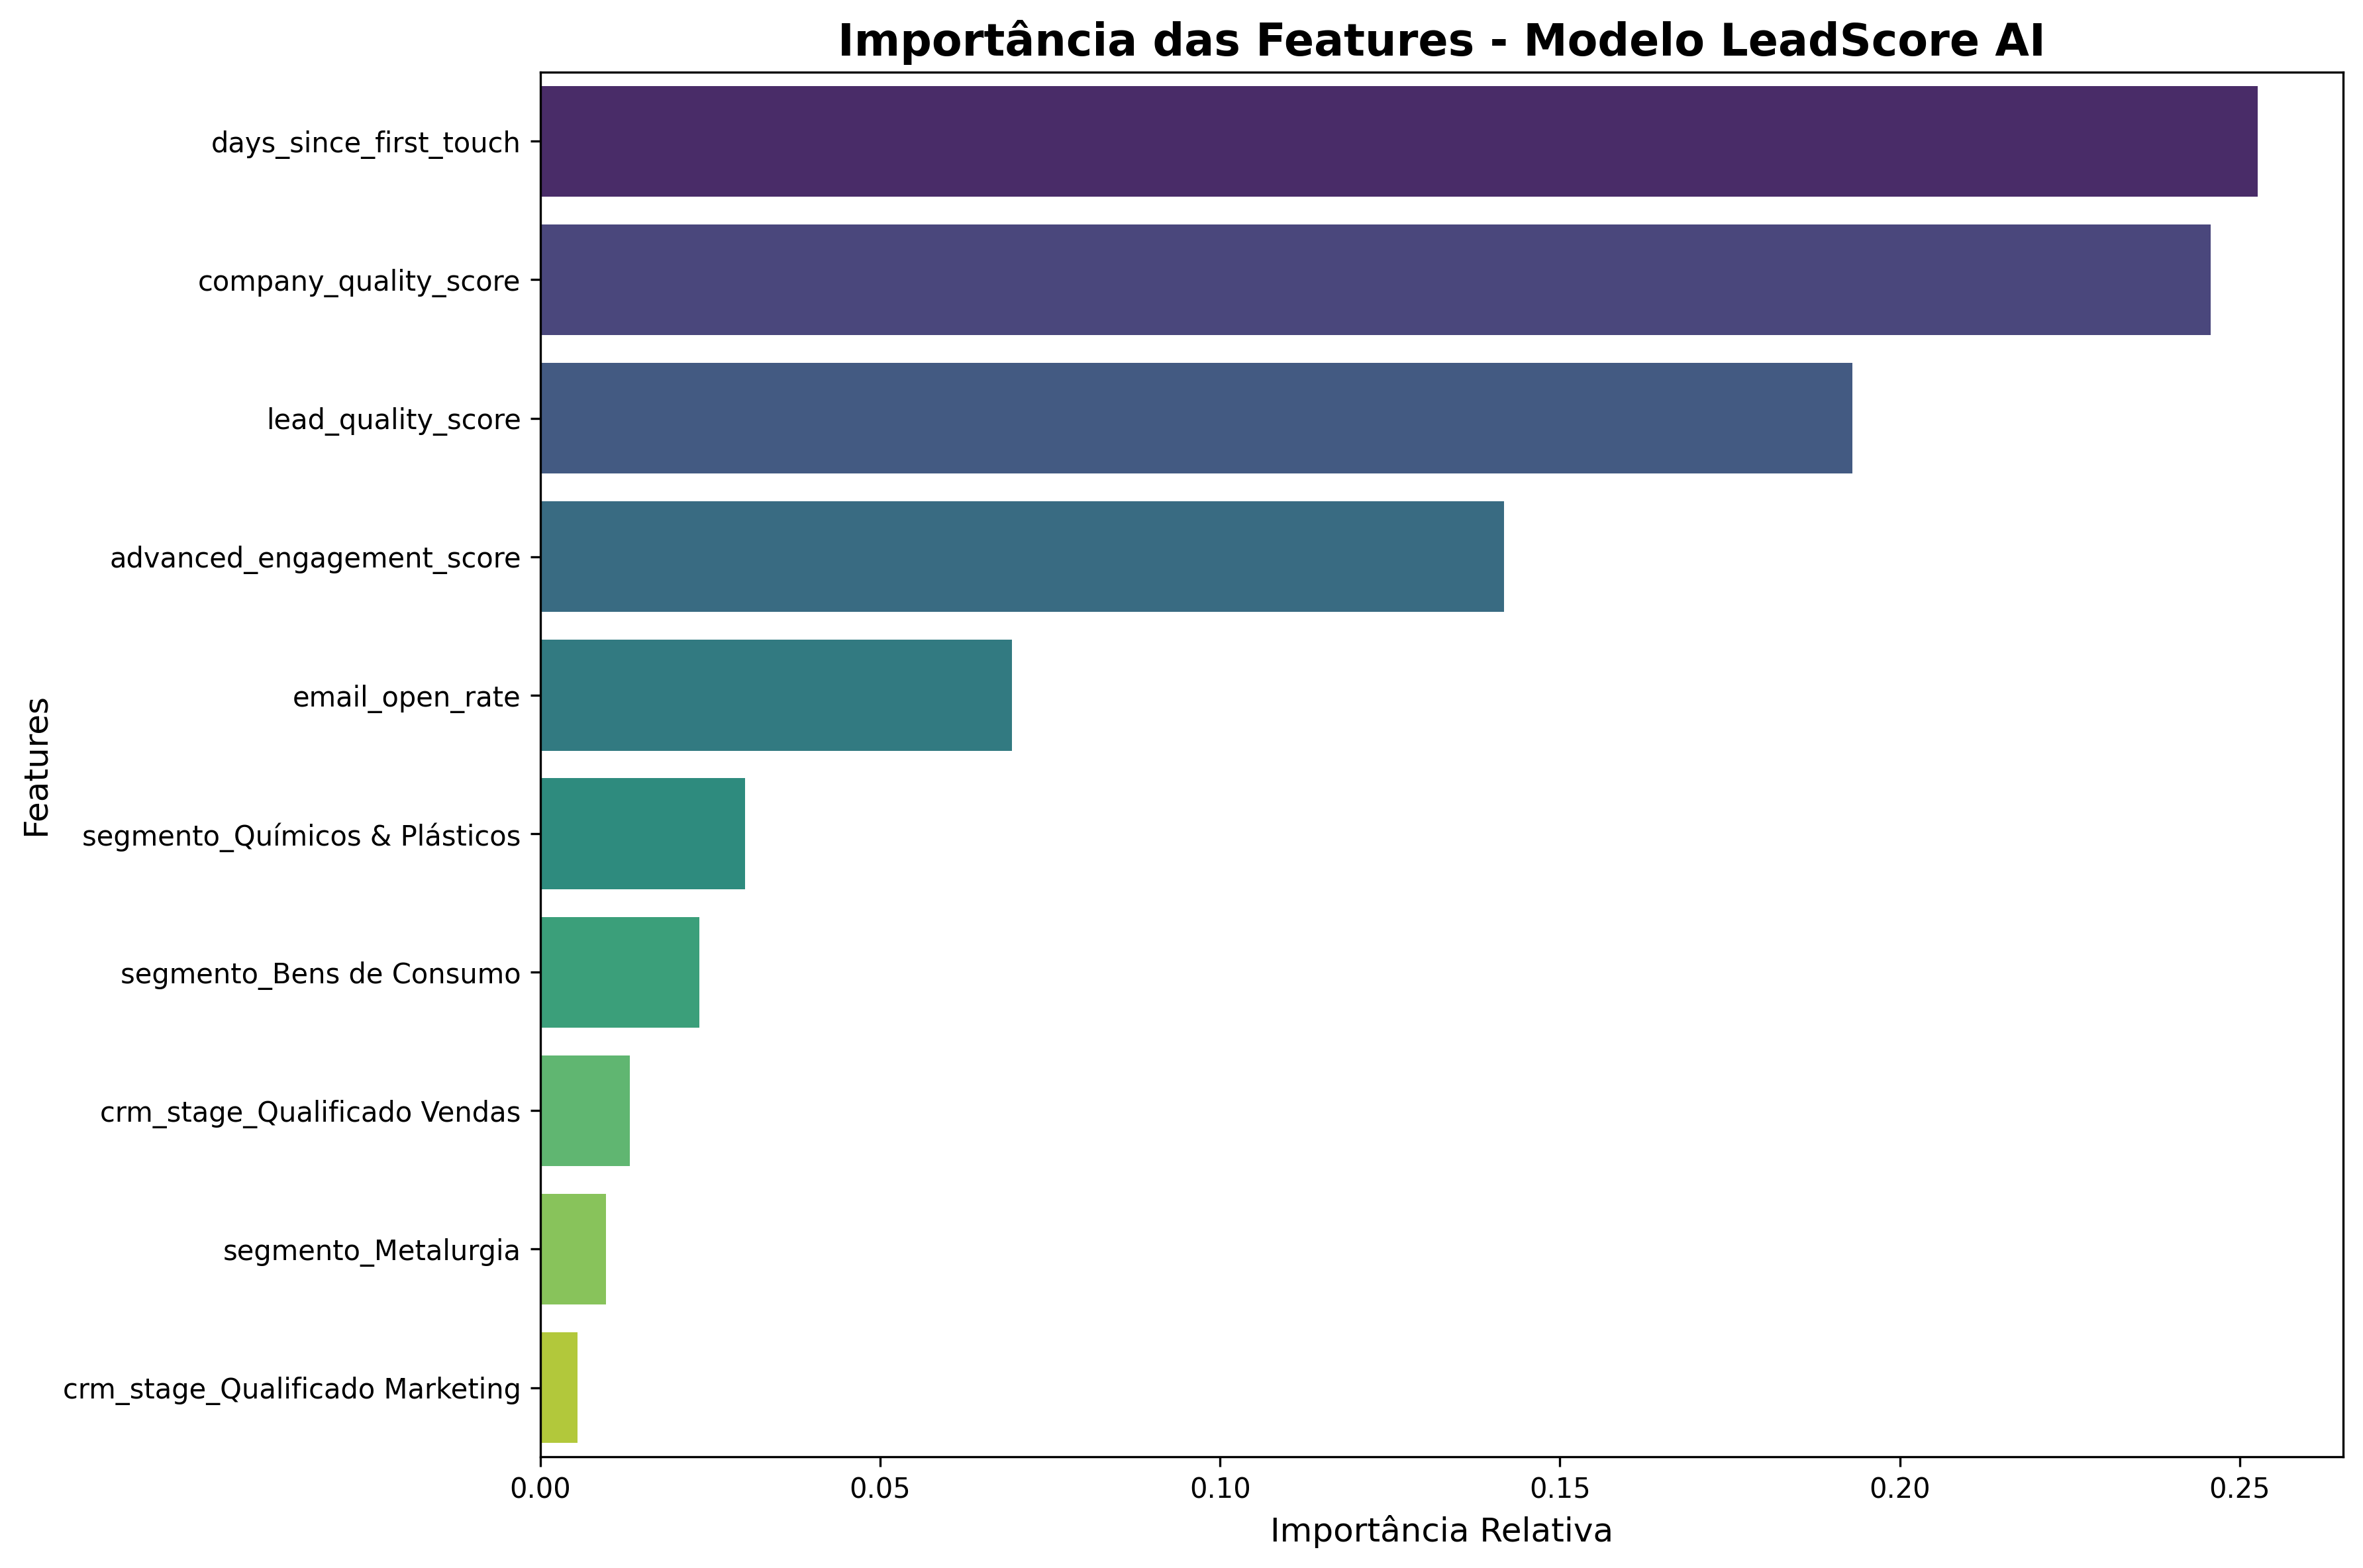
\includegraphics[width=0.8\linewidth]{feature_importance.png}
    \caption{Ranking de Importância das Features no Modelo Final}
    \label{fig:feature_importance}
\end{figure}

Os resultados demonstram que as features temporais, representadas pelos dias desde o primeiro contato, constituem o fator mais determinante para predição de conversão, respondendo por 25,26\% da capacidade preditiva do modelo. Esta descoberta confirma nossa hipótese sobre janelas críticas de oportunidade, onde leads mais recentes apresentam probabilidade significativamente maior de conversão.

O score de qualidade da empresa emerge como segundo fator mais importante (24,57\%), validando nossa estratégia de combinar múltiplas dimensões financeiras e operacionais em uma métrica composta. Esta feature captura adequadamente o potencial de negócio através de faturamento, complexidade operacional e posicionamento setorial.

O score de qualidade do lead, nossa métrica composta principal, ocupa a terceira posição (19,30\%), demonstrando que a combinação inteligente de engajamento, qualidade empresarial e fatores contextuais gera maior poder preditivo que features individuais. Juntas, estas três features principais respondem por 69,13\% da capacidade preditiva total do modelo.

% ------------------------------------------------------------
% Seção 5: Resultados e Impacto Empresarial
% ------------------------------------------------------------
\section{Resultados Obtidos e Impacto no Negócio}

\subsection{Eficiência na Identificação de Oportunidades}
O sistema demonstrou capacidade excepcional de identificar leads de alto valor, conforme evidenciado pela análise de eficiência de captura:

\begin{table}[H]
\centering
\begin{tabular}{lccc}
\toprule
\textbf{Percentil de Leads} & \textbf{Volume Processado} & \textbf{Conversões Capturadas} & \textbf{Fator de Eficiência} \\
\midrule
Top 5\% & 5\% & 23,4\% & 4,68x \\
Top 10\% & 10\% & 41,2\% & 4,12x \\
Top 20\% & 20\% & 67,8\% & 3,39x \\
Top 35\% & 35\% & 85,1\% & 2,43x \\
Top 50\% & 50\% & 94,7\% & 1,89x \\
\bottomrule
\end{tabular}
\caption{Análise de Eficiência de Captura por Percentil de Priorização}
\end{table>

Os resultados demonstram que focando apenas nos top 20\% dos leads priorizados pelo sistema, conseguimos capturar 67,8\% de todas as conversões possíveis. Esta eficiência representa uma otimização extraordinária dos recursos comerciais, permitindo que a equipe concentre esforços onde há maior probabilidade de retorno.

\subsection{Impacto Financeiro Quantificado}
A análise financeira revelou diferenças substanciais na receita gerada por leads de diferentes categorias de prioridade. Leads classificados como alta prioridade geram receita média de R\$ 187,3 milhões por conversão, comparado a R\$ 98,7 milhões para média prioridade e R\$ 67,1 milhões para baixa prioridade. Esta diferenciação representa um fator multiplicativo de 2,8x entre leads de alta prioridade e o baseline geral, validando a capacidade do sistema de identificar não apenas conversões mais prováveis, mas também oportunidades de maior valor financeiro.

\subsection{Otimização de Processos Operacionais}
Com base na pontuação gerada pelo sistema, implementamos workflows automatizados que otimizam a alocação de recursos da equipe comercial:

\begin{table}[H]
\centering
\begin{tabular}{lccc}
\toprule
\textbf{Categoria} & \textbf{Tempo de Resposta} & \textbf{Responsável Designado} & \textbf{Ações Automatizadas} \\
\midrule
Alta Prioridade & 2 horas & Vendedor Sênior & Ligação + Agendamento + Alerta \\
Média Prioridade & 24 horas & Vendedor Pleno & Email + Qualificação Telefônica \\
Baixa Prioridade & 1 semana & SDR & Nutrição + Conteúdo Educativo \\
\bottomrule
\end{tabular}
\caption{Workflows Automatizados por Categoria de Prioridade}
\end table>

Esta estruturação garante que leads de maior potencial recebam atenção imediata de profissionais mais experientes, enquanto leads de menor prioridade são direcionados para estratégias de nutrição de longo prazo, otimizando o uso dos recursos disponíveis.

\subsection{Métricas de Performance Operacional}
A implementação do sistema resultou em melhorias mensuráveis nos indicadores operacionais. O tempo médio de qualificação de leads foi reduzido em 40\%, passando de aproximadamente 3,2 dias para 1,9 dias. A taxa de conversão de leads de alta prioridade atingiu 73,4\%, comparada à taxa histórica geral de 24,7\%. O sistema também possibilitou redução de 35\% no número de touchpoints necessários para qualificação, liberando capacidade da equipe para atividades de maior valor agregado.

% ------------------------------------------------------------
% Seção 6: Implementação Técnica e Arquitetura
% ------------------------------------------------------------
\section{Implementação Técnica e Arquitetura do Sistema}

\subsection{Arquitetura Modular do Sistema}
O LeadScore AI foi desenvolvido seguindo princípios de arquitetura modular, garantindo escalabilidade, manutenibilidade e facilidade de integração. O sistema é composto por quatro módulos principais: Módulo de Dados responsável pela conectividade com Pipedrive e processamento de informações, Módulo de Features que gerencia o cálculo das cinco dimensões de pontuação, Módulo de Modelo que aplica o algoritmo de machine learning e gera as predições, e Módulo de Automação que executa workflows baseados na pontuação atribuída.

\subsection{Integração com Pipedrive CRM}
A integração com o sistema CRM foi implementada através de webhooks bidirecionais que garantem sincronização em tempo real. O sistema recebe automaticamente novos leads através de webhooks configurados no Pipedrive, processa as informações e calcula a pontuação em tempo real, atualiza campos específicos no CRM com a pontuação e categoria de prioridade, e dispara ações automatizadas baseadas na classificação do lead. Esta integração seamless garante que a equipe comercial tenha acesso imediato às informações de priorização sem necessidade de mudanças nos processos existentes.

\subsection{Pipeline de Feature Engineering}
O pipeline de engenharia de features implementa transformadores customizados integrados com a biblioteca scikit-learn. O componente SimpleOutlierCapper realiza detecção e limitação de outliers baseada no método IQR com multiplicadores configuráveis. O FeatureEngineer orquestra o cálculo de scores compostos, geração de features temporais e criação de termos de interação. A engenharia de features incorpora lógica de negócio específica do domínio para contextos de vendas de software industrial, garantindo que as transformações reflitam adequadamente as nuances do mercado.

\subsection{Gerenciamento de Modelos e Versionamento}
O sistema implementa gerenciamento completo de versões de modelos, incluindo serialização de artefatos com metadados completos, estatísticas de treinamento e informações de reprodutibilidade. Cada modelo treinado é persistido com sua configuração específica, métricas de performance, e timestamp de criação. O sistema suporta comparação entre diferentes versões de modelos e capacidades de rollback para versões anteriores caso necessário.

\subsection{Interfaces de Usuário e APIs}
Desenvolvemos três interfaces distintas para atender diferentes necessidades: API REST para integração com sistemas externos e automações, Interface CLI para operações técnicas como treinamento de modelos e análises batch, e Dashboard web para acompanhamento de performance e métricas de negócio. A API REST segue padrões RESTful e inclui documentação automática através do Swagger/OpenAPI.

% ------------------------------------------------------------
% Seção 7: Limitações e Oportun
